\documentclass[]{article}
\usepackage[a4paper, total={6in, 10in}]{geometry}
\usepackage{hyperref}
\usepackage{amsmath}
\usepackage{graphicx}
\usepackage[outdir=./]{epstopdf}
\usepackage{booktabs}
\usepackage{float}
\usepackage{subcaption}

\setlength{\parindent}{0em}
\setlength{\parskip}{1em}

\DeclareMathOperator{\cov}{cov}

%opening
\title{SSY 230, System Identification\\
	Project 3: Identification of a Real System}
\author{Yuxuan Xia\\ \href{mailto:yuxuan.xia@chalmers.se}{yuxuan.xia@chalmers.se}\\Emil Staf\\\href{mailto:emil.staf@chalmers.se}{emil.staf@chalmers.se}}

\begin{document}

\maketitle


\section{Flexible Robot Arm}
The system we have chosen to identify is a mechanical system, where a flexible robot arm have been installed on an electrcal motor. It is a SISO system where the input $u(t)$ is measured reaction torque and the output $y(t)$ is the acceleration of the flexible robot arm. The experimental set-up was performed using a periodic sinusodial sweep.

\subsection{Data}
As mentioned previously the input data is a periodic sinusodial sweep (see top plot of Figure \ref{fig:input}). Due to the fact that the data was obtained using a periodic sinusodial sweep we split the data in half and use the first part as training data and the second part as validation data.

\begin{figure}[ht]
\centering
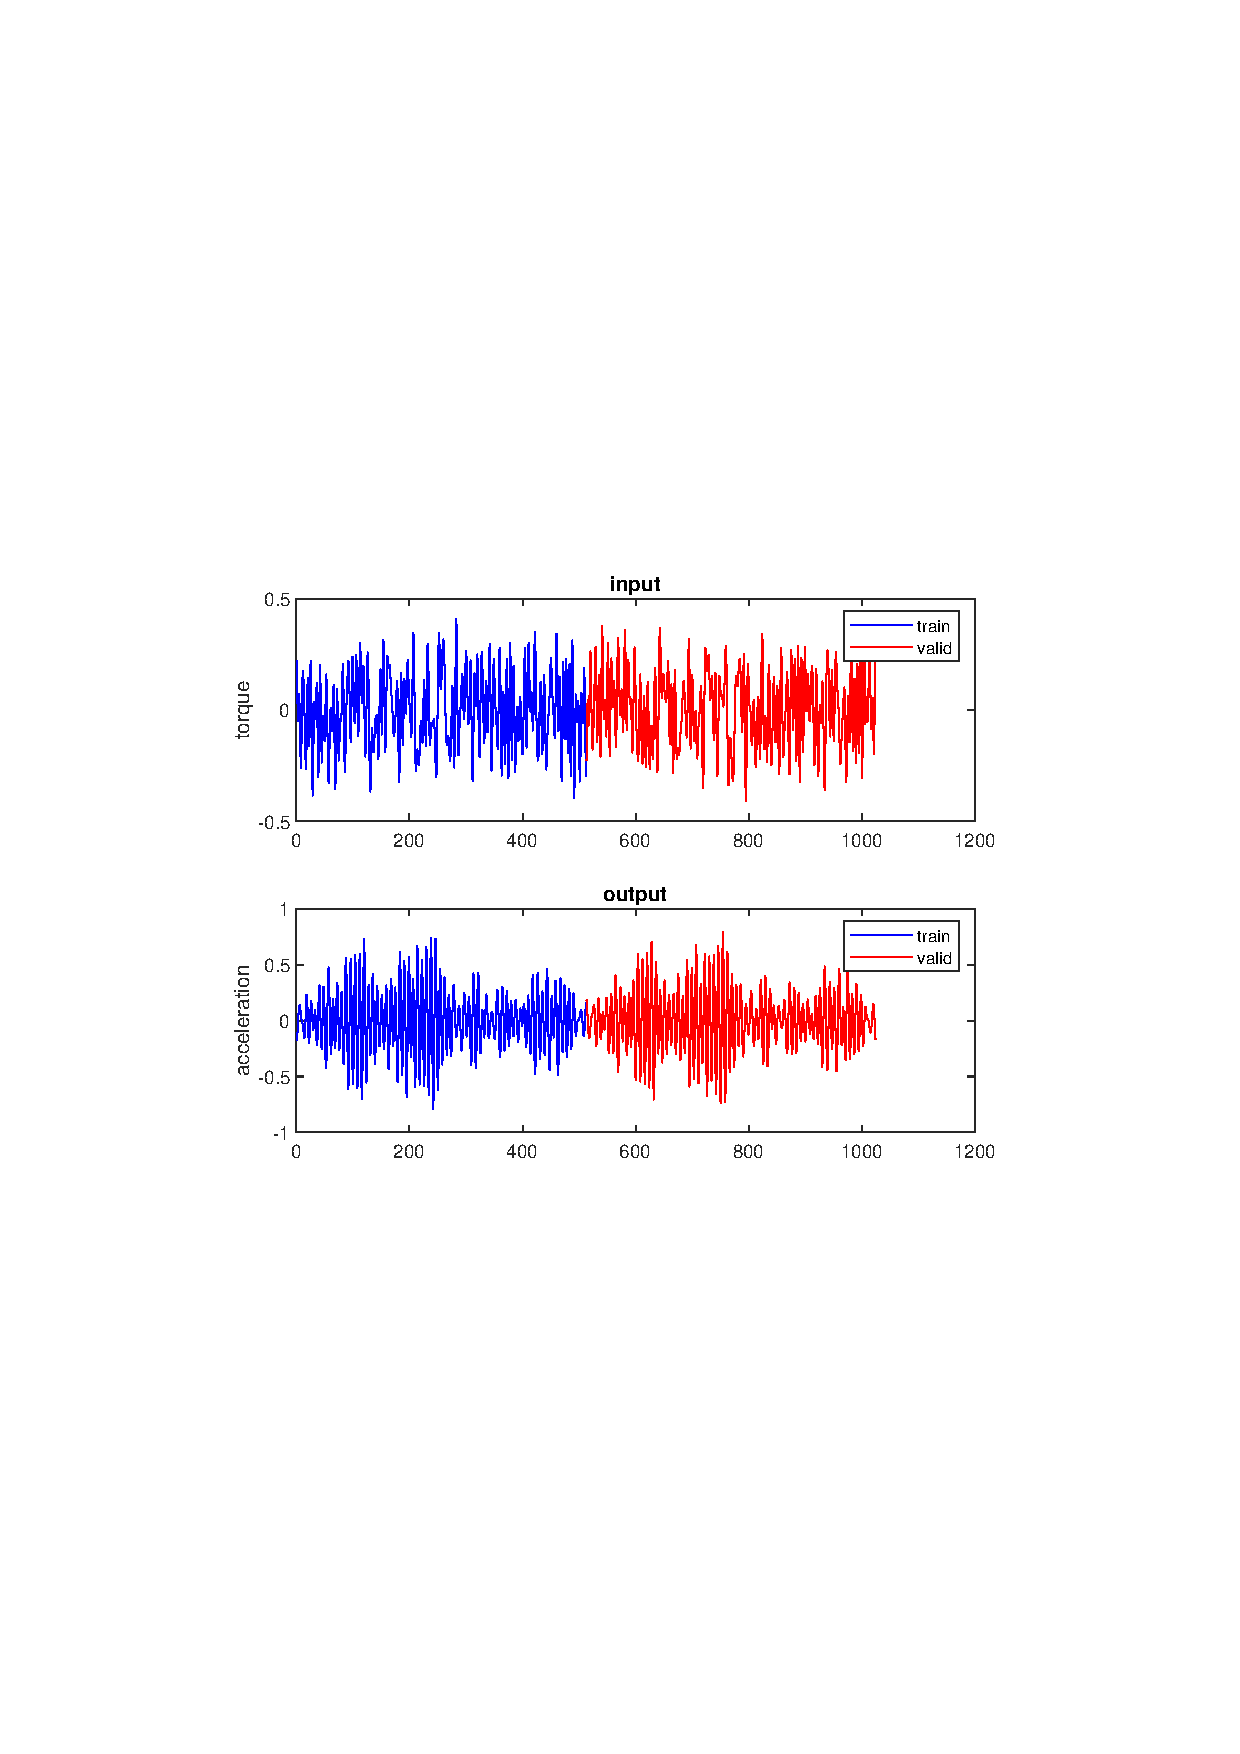
\includegraphics[trim= 10cm 8cm 10cm 8cm, scale=0.7]{figures/input.pdf}
\caption{System data, input $u(t)$ (top) and output $y(t)$ (bottom).}
\label{fig:input}

\end{figure}
To make sure that the frequency content in both the training and validation data are similar we use the \emph{etfe} in MATLAB to find the Empirical Transfer Function Estimate of training- and validation data. The resulting bode-plot is shown in Figure \ref{fig:bode-train_valid}.

\begin{figure}[ht]
\centering
\begin{subfigure}{.49\textwidth}
	\centering
	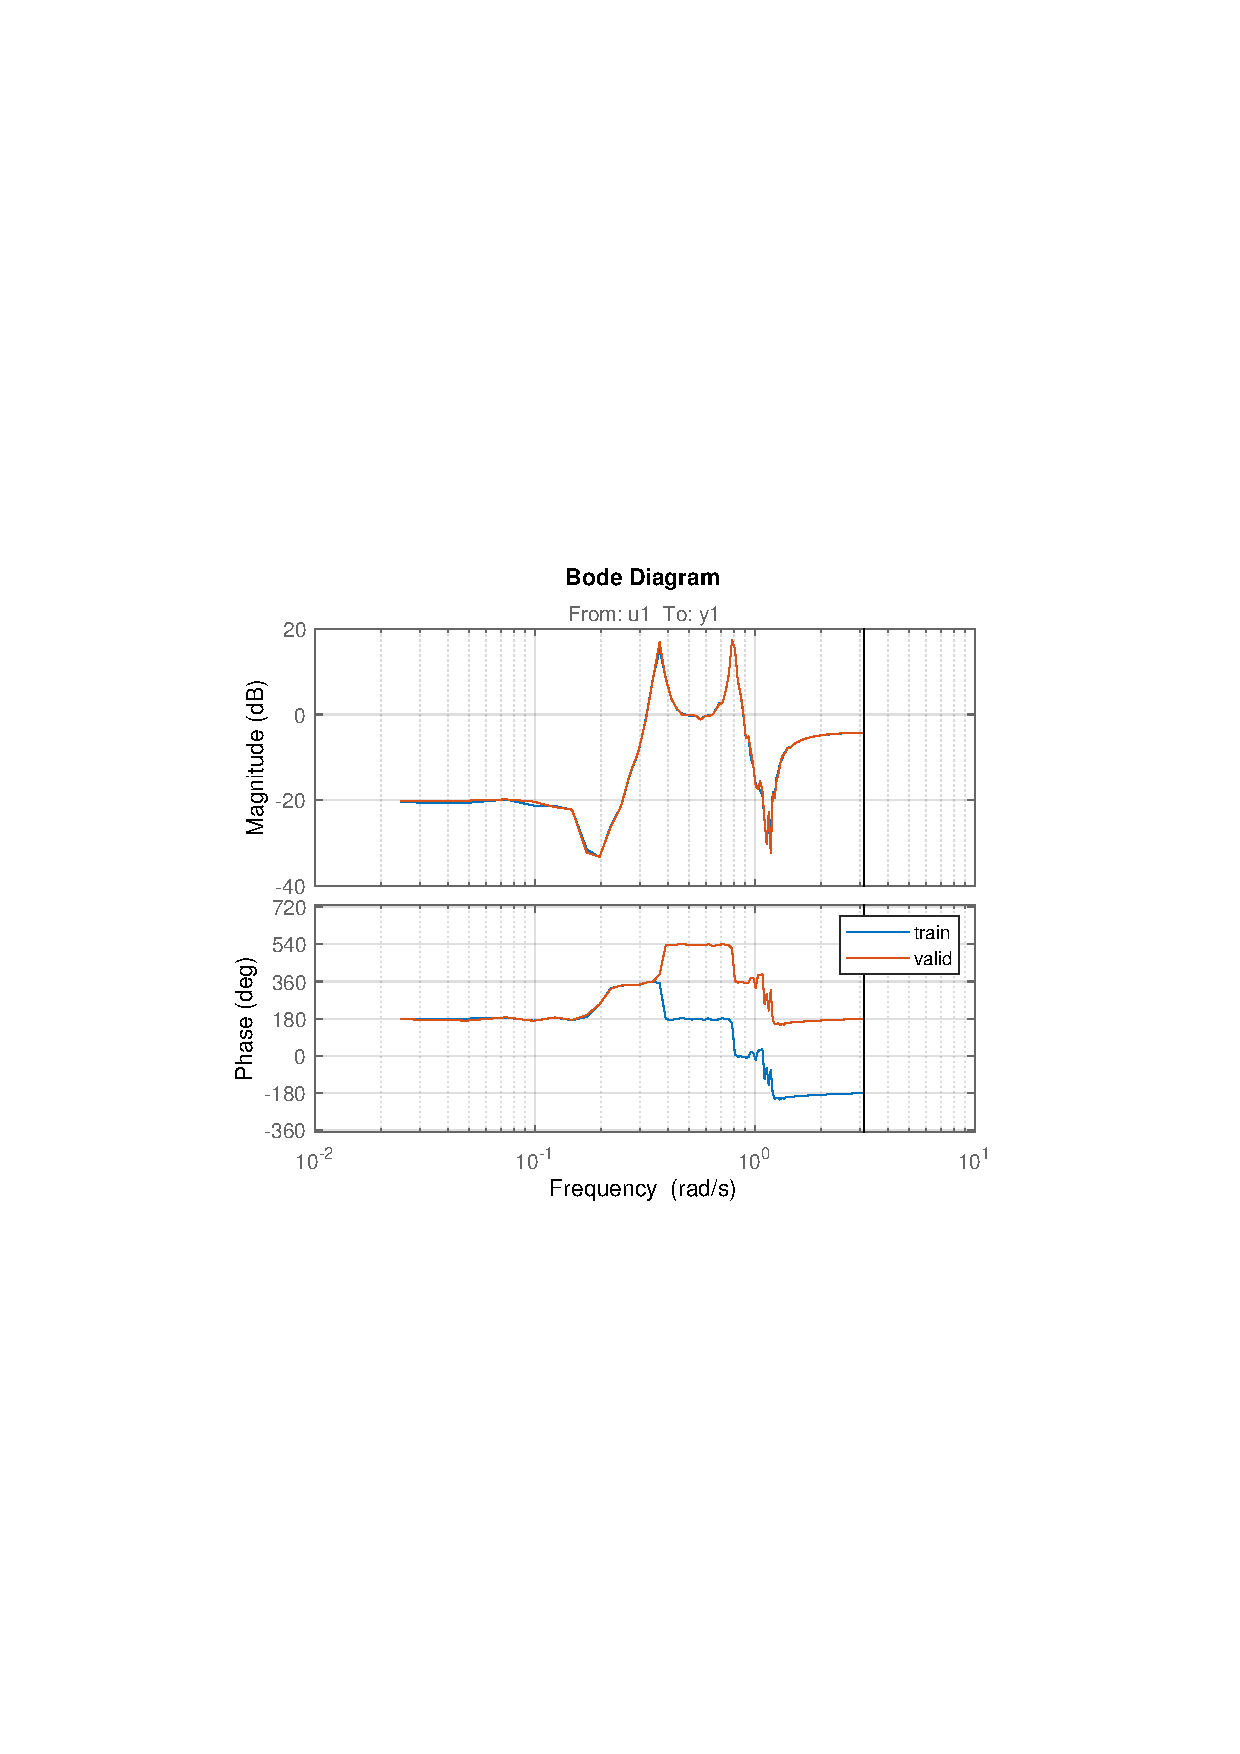
\includegraphics[trim= 10cm 8cm 10cm 8cm, scale=0.4]{figures/bode-train_valid.pdf}
	\caption{Bode-plot of training and validation data.}
	\label{fig:bode-train_valid}
\end{subfigure}
\begin{subfigure}{.49\textwidth}
	\centering
	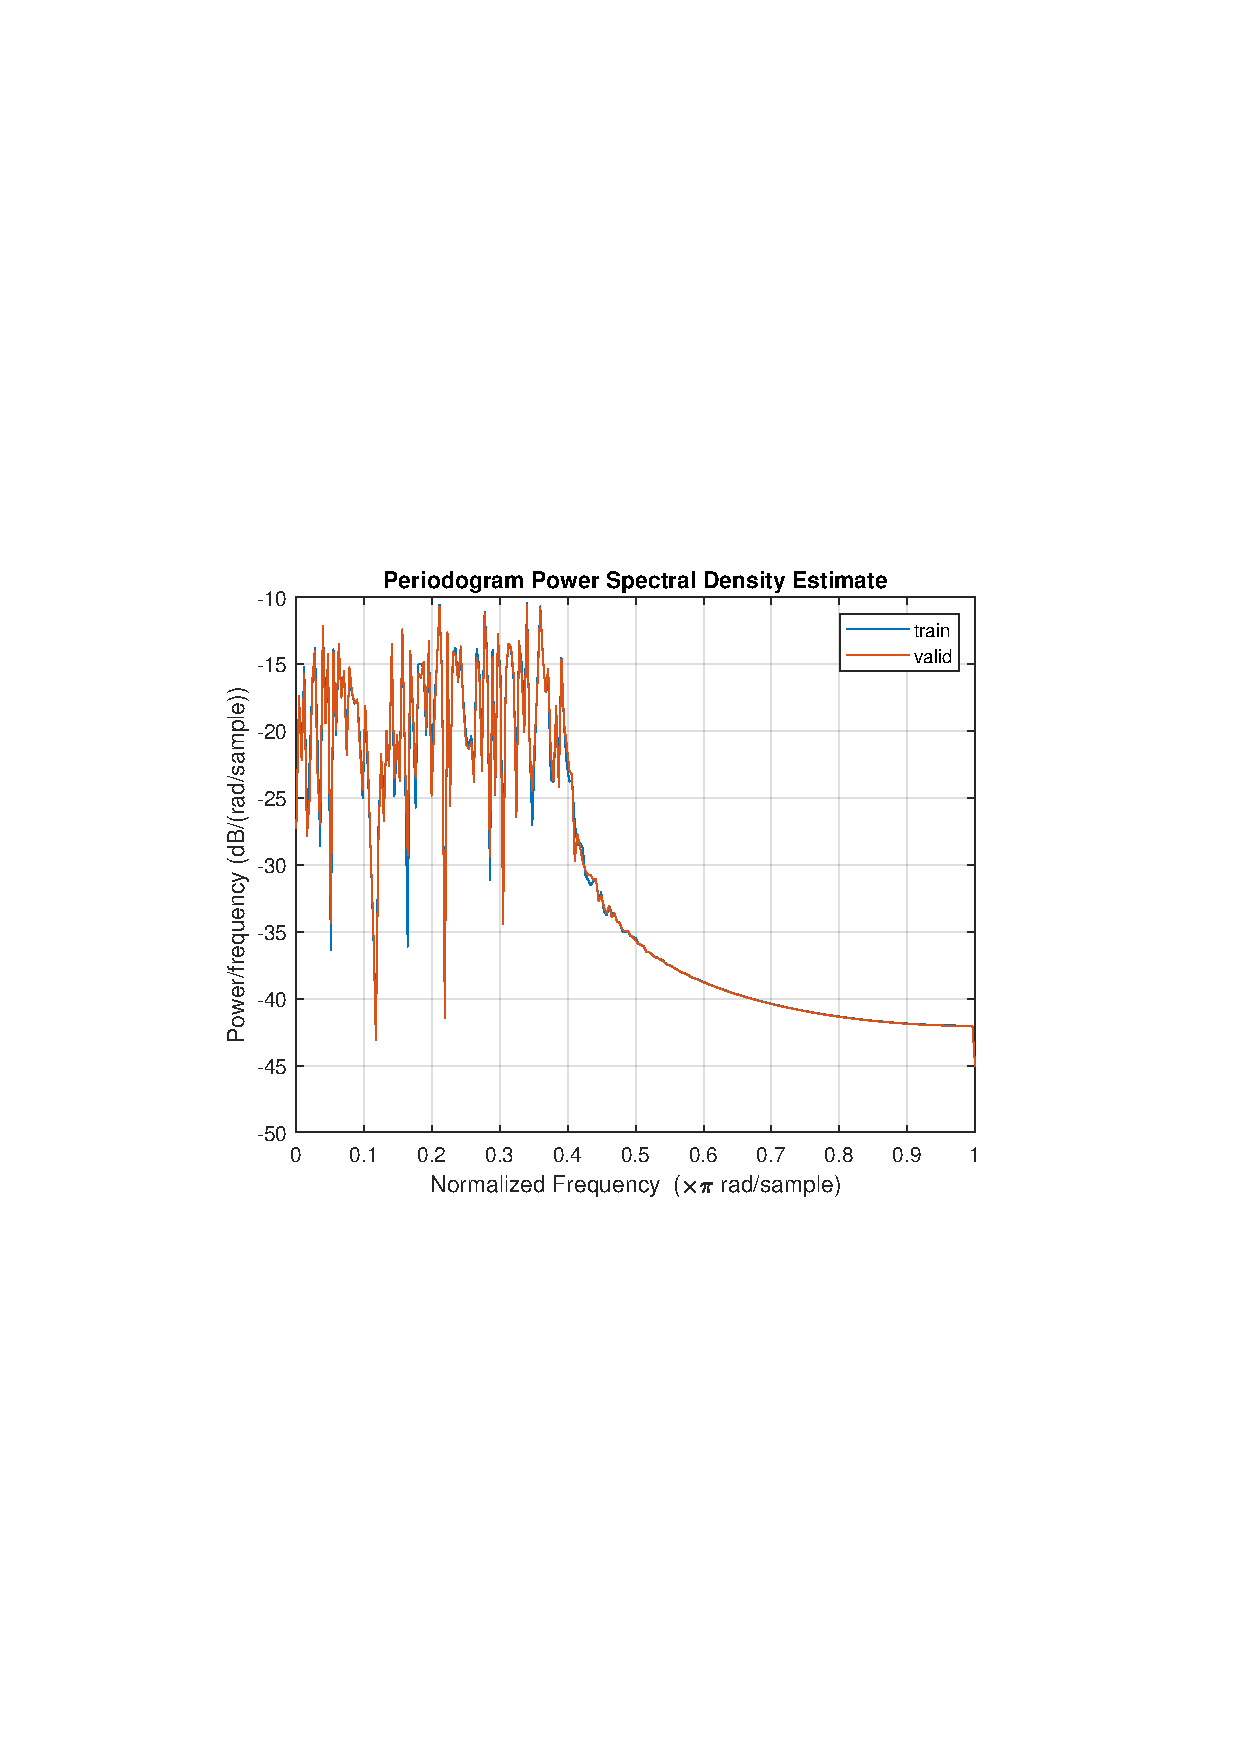
\includegraphics[trim= 10cm 8cm 10cm 8cm, scale=0.4]{figures/periodogram-train_valid.pdf}
	\caption{Periodogram of training and validation data.}
	\label{fig:periodogram-train_valid}
\end{subfigure}
\caption{Analyzing training/validation split.}
\label{fig:train_valid}
\end{figure}

From analysing Figure \ref{fig:bode-train_valid} it is clear that the amplitude of the frequency content in both training- and validation data is very similar, while there is a 360 degree phase shift approximately starting from frequencies $>0.35$ rad/s. However, it should be noted that a 360 degree phase shift means the validation data and training data are still in phase. Using the MATLAB build-in function \emph{periodogram} it is clear that the frequency content of the training- and validation data is very similar and we conclude that the chosen way to construct training/validation data is a good choice.

It can be interesting to analyse the autocorrelations of and cross-correlation between the input $u(t)$ and the output $y(t)$. The correlations can be seen in Figure \ref{fig:cross-correlation}.
\begin{figure}[ht]
\centering
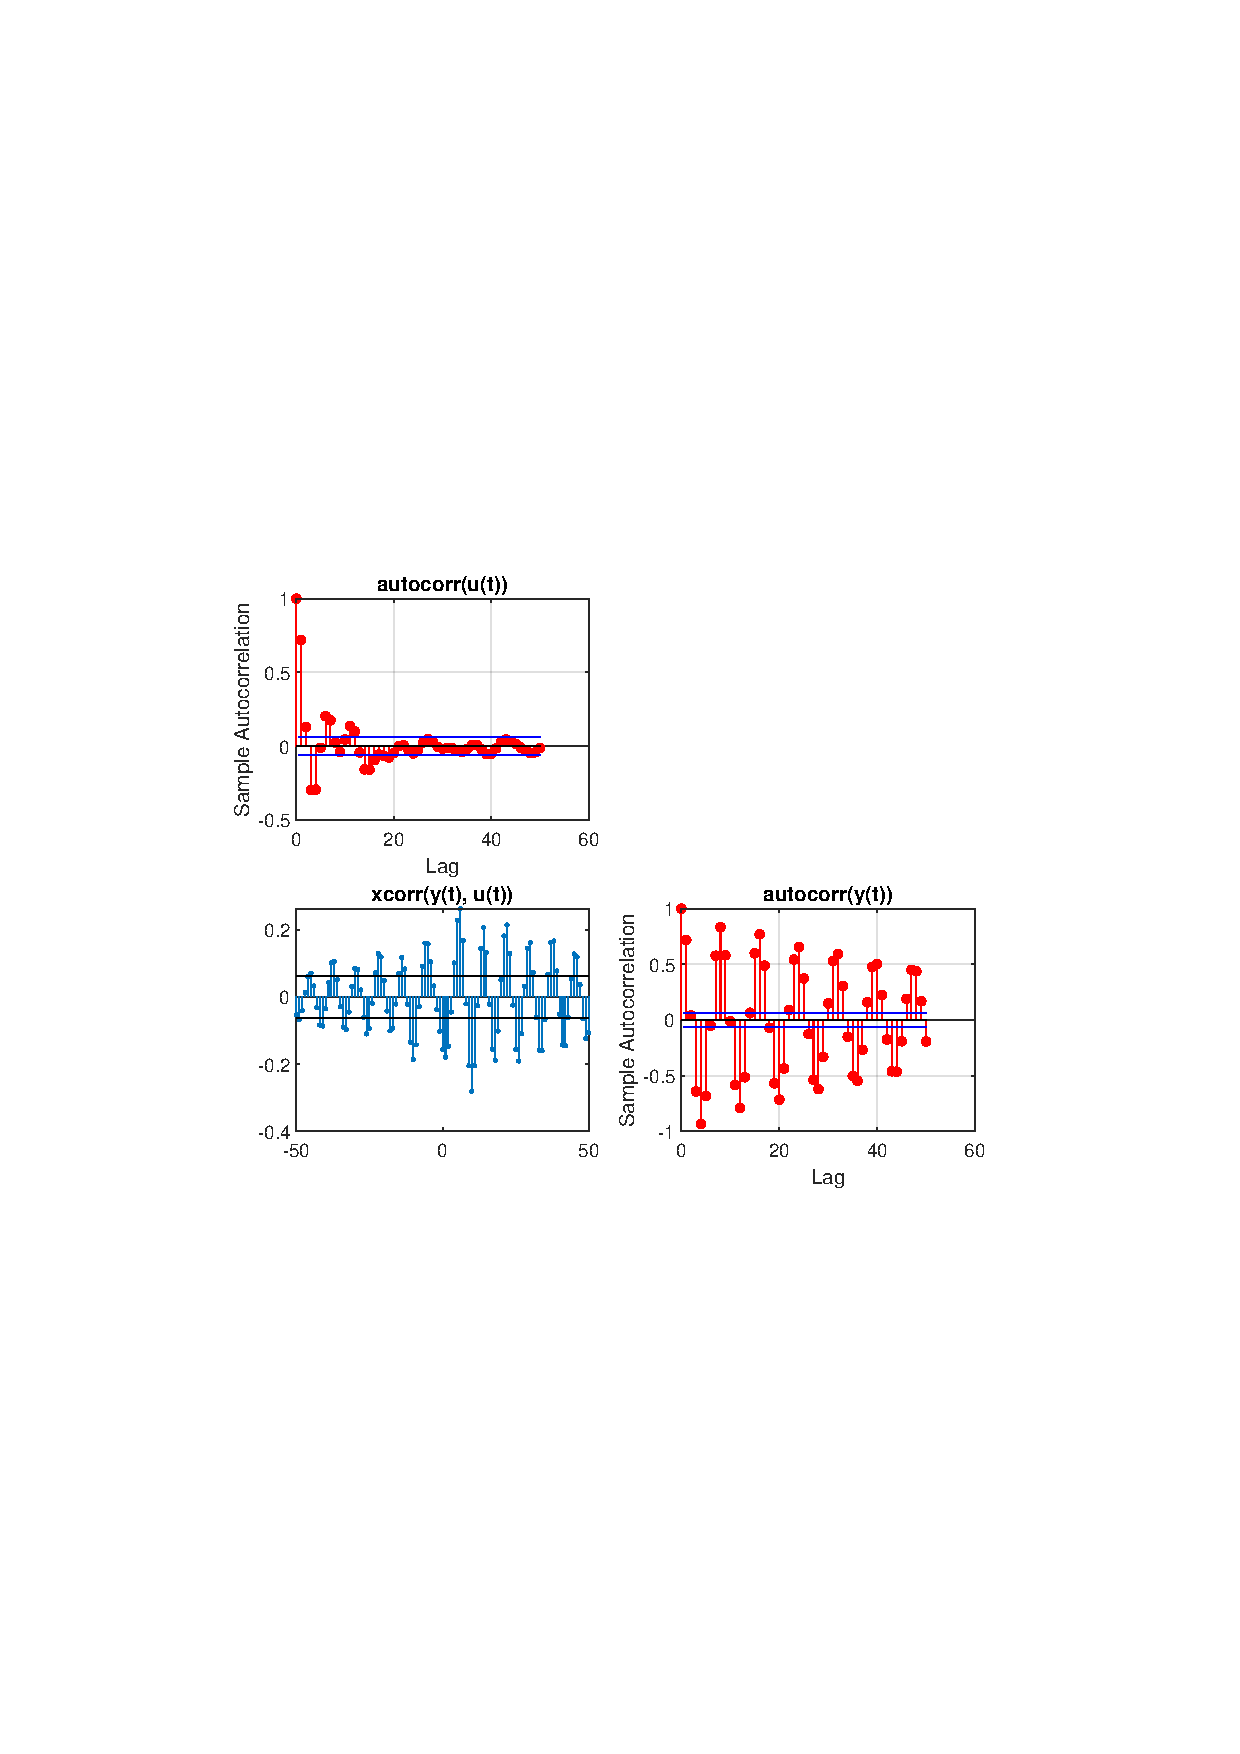
\includegraphics[trim= 10cm 8cm 10cm 8cm, scale=0.7]{figures/cross-correlation.pdf}
\caption{Autocorrelations of and cross-correlation between the input $u(t)$ and the output $y(t)$}
\label{fig:cross-correlation}
\end{figure}
From Figure \ref{fig:cross-correlation} it is clear that the output depends on previous values of itself as well as previous values of the input. 

\textbf{NOTE:} We should return to cross-correlation analysis after having a trained model of the system to make sure there are no cross-correlations remaining, since that could mean that a too simple model would have been used.

\subsection{Pre-Processing}


\end{document}
